% !TEX root = ../Thesis.tex
% !TEX spellcheck = en-US

\chapter{Introduction}
\label{ch:introduction}

This first chapter introduces the challenge of using virtual, fully software-based alternatives to computer network labs in education, with special emphasis on the undergraduate and graduate levels of the university. % TODO should university by capitalized here?
It also proposes the definitions that, though not universal or unique, help precise differences between those software solutions, namely two main concepts: simulation and emulation. % TODO universal NOR unique?
Together with the last point, this chapter also explains the reason why this thesis is centered, starting from its title, in ``emulators'' more than on ``simulators''.
Finally, it gives a very brief overview of the work that has already been done in the field of computer networks simulators and emulators, and, orthogonally, in the replacement of laboratories with (physical) hosts and routers/switches in schools and universities by simulated or emulated (virtual) solutions.

% end of intro

\section{Motivation and problem statement}
\label{sec:motivation}

On most education institutions, computer networks teaching has used physical laboratories, making it possible for students to exercise experimentally the knowledge acquired in the theoretical component of subjects whose program envisions going beyond skills strictly related to programming exercises---i.e. that involves contact with real networks and concrete equipment.
The existence of those laboratories is, even today, standard practice in many institutions of higher education. FCT/NOVA, which is not an exception, has a room with routers and switches for performing those practical exercises.

Despite its virtues, starting with responding to a pedagogical need in the teaching of Engineering for applying the learned theory and getting ``hands on'' experience, this method raises problems such as the cost and fast obsolescence~\cite{automaticnetconfiggns} of equipments, the demand for individual presence on the laboratory (at least for manipulating physical links and network interfaces) for exercise elaboration, the possible damage due to misuse~\cite{teachinginovation} or simple wear-and-tear, the time and effort to prepare and setup for given exercises, which may even ``destroy'' the setup for other exercises, etc. % TODO avoid repeating "exercise" so much here

Aiming to address these problems, not exclusive from further or higher education, extending to vocational education on high schools and ``\emph{politécnicos}'', and even ``courses'' of the industry itself, of which Cisco's CCNA~\cite{ccna} is a good example, or even distance learning, tools for emulating and/or simulating networks and networking equipment have been developed for years. % TODO replace "extending". o "vocational education" veio do linguee
These tools can, through the usage of several techniques, surpass some (if not all) of the aforementioned disadvantages.

\subsection{The lab on a laptop}
\label{subsec:replacingthelab}

% end of subsec replacingthelab

\subsection{Emulation, simulation (and virtualization)}
\label{subsec:emulsimvirt}

% end of subsec emulsimvirt

% end of section motivation

\section{Related work}
\label{sec:relatedwork}

% PROBABLY SOME SUBSECTIONS GO HERE

% \subsection{The lab on a laptop}
% \label{subsec:replacingthelab}

% % end of subsec replacingthelab

% \subsection{Emulation, simulation (and virtualization)}
% \label{subsec:emulsimvirt}

% % end of subsec emulsimvirt

% end of section gns3performance

\begin{figure}
  \centering
  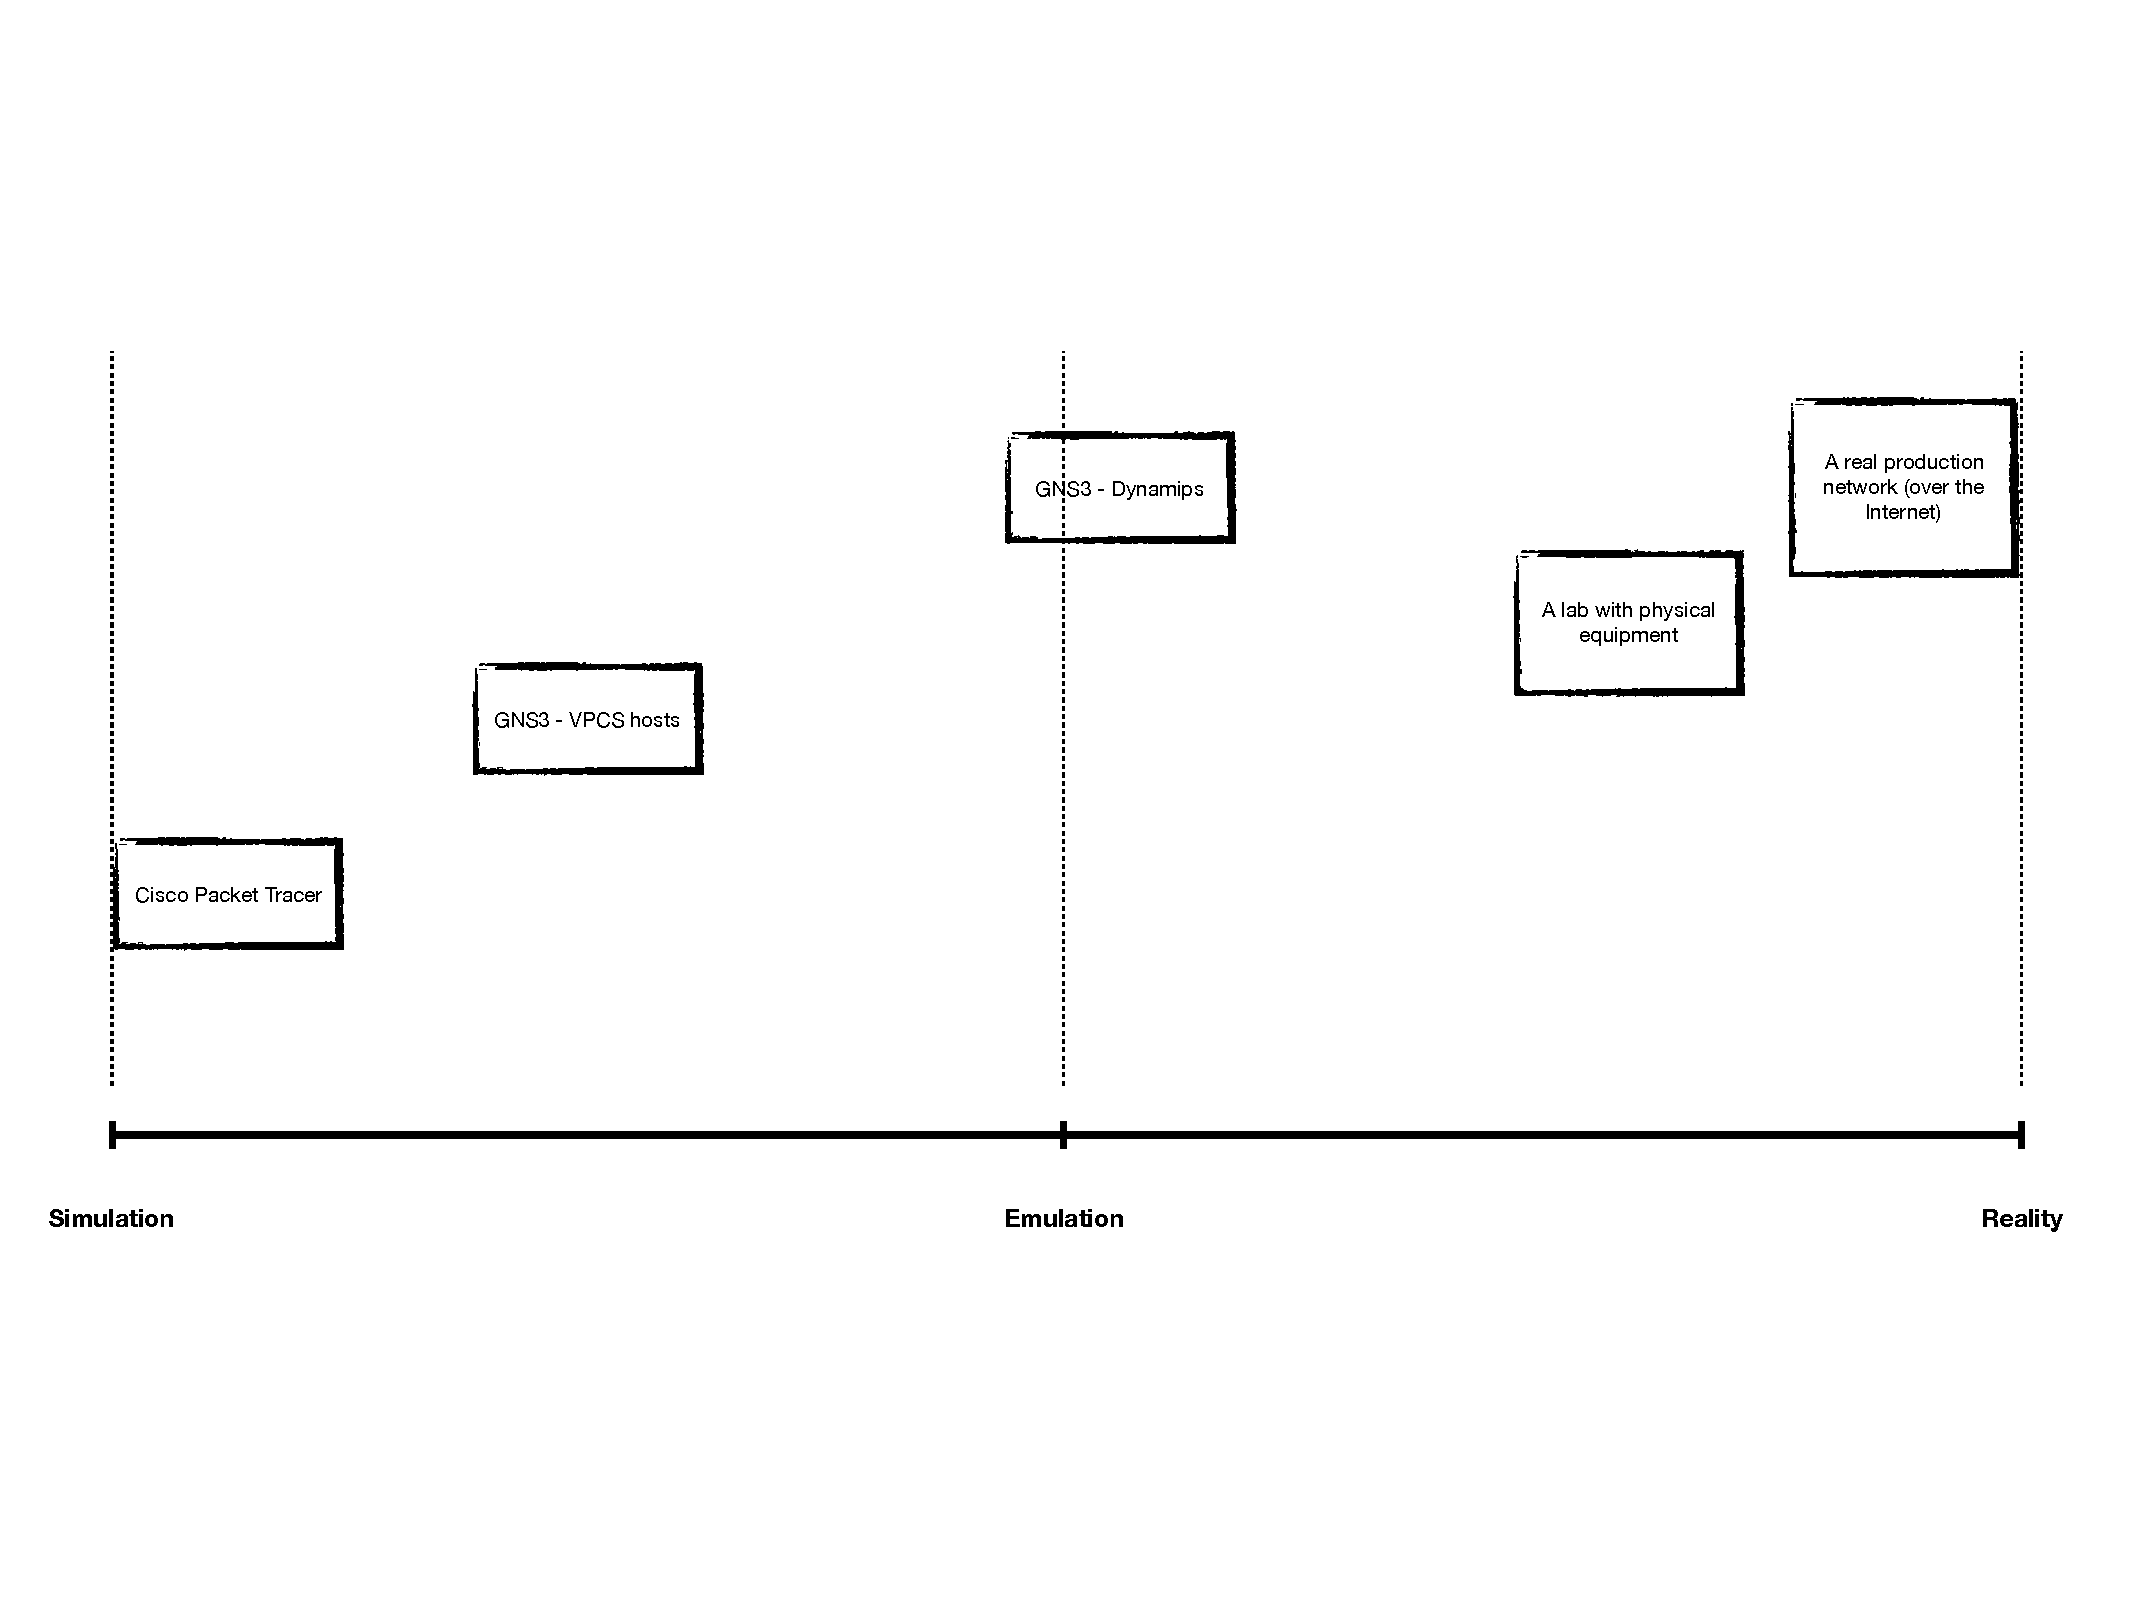
\includegraphics[width=0.8\textwidth]{emulationvsreality}
  \caption{Simulation vs emulation vs reality}
  \label{fig:emulationvsreality}
\end{figure}

% \section{The first section of this intro}
% Here we can comment on the super-interesting aspects of the diagram depicted in figure~\ref{fig:emulationvsreality}.

\section{Structure of the thesis}
\label{sec:structure}

% end of section structure

% end of chapter
